\documentclass[11pt]{article}

\usepackage[utf8]{inputenc}
\usepackage[T1]{fontenc}
\usepackage{lmodern}
\usepackage{enumitem}
\usepackage[left=2.5cm,right=2.5cm]{geometry}
\usepackage{xcolor}
\definecolor{navy}{RGB}{17,85,170}
\usepackage{amsmath}
\usepackage{amssymb}
\usepackage{graphicx}
\usepackage{booktabs}
\usepackage{subcaption}
\usepackage{tabularx}
\usepackage{colortbl}
\newcolumntype{Z}{>{\hsize=.4\hsize}X}
\usepackage{ragged2e}
\usepackage[font=footnotesize,justification=justified,singlelinecheck=false]{caption}
\captionsetup[subfigure]{justification=centering,singlelinecheck=true}
\usepackage{natbib}
\usepackage{currfile}
\usepackage{xr-hyper}
\usepackage{hyperref}
\externaldocument[][nocite]{../main} % nocite: do not import the paper's citation keys (the letter has its own bibliography)
\newcommand{\comment}[1]{\begingroup #1\endgroup}
\newcommand{\answer}[1]{\begingroup\color{navy}#1\endgroup}

%\author{}
\title{Response to Referee 3 (EJ MS20241010-2)}
\date{}

\begin{document}
%\maketitle

\begin{center}
   \LARGE{Response to Referee 3 (EJ MS20241010-2)}
\end{center}

\vspace{0.5em}
\noindent \answer{We thank the referees and the editor for their time and thoughtful feedback. We have revised the paper to address all of the comments raised. We respond below point by point, in blue. To ease the reading, we report all revised Figures and Tables in the appendix of this letter. We also directly quote the revised text in italics.}\par

% \section*{Roadmap on main empirical changes}

\answer{Answer TBW.

%\begin{enumerate}[leftmargin=*]
%\item \textbf{...}
%\end{enumerate}
}

\par
\vspace{0.5em}


\section*{Evaluation}
\comment{
I found the revision convincing and substantially improved relative to the previous version. The authors have carefully addressed the main concerns raised in my report, including the definition of displaced workers, the comparison with the mass-layoff literature, the measurement of firm characteristics, and the discussion of the implications for structural models. The paper now provides clear and compelling evidence on the reallocation of displaced workers across firms and makes a valuable contribution to the literature. The comments below are relatively minor and mainly aimed at improving clarity.
}\par


%\answer{Thank you for your kind words and thoughtful feedback. We have revised the paper to address all of your comments.}\par

\section*{Comments}


\begin{enumerate}[leftmargin=*]
\item[1.] 
\comment{\textbf{Descriptive statistics}. I may have missed it, but I found it surprisingly difficult to locate a simple descriptive table summarizing the treated and comparison groups before displacement. At a minimum, I would encourage the authors to report predisplacement means of the main outcome variables (earnings, hourly wages, and hours worked). This would help readers assess economic magnitudes and facilitate comparisons with the broader displacement literature.
}\par

\answer{We agree that this table should be easier to find. In the previous version, it was Appendix Table A4, referred to in Section~\ref{sec:stat_desc}. It reports, for displaced workers (column 1) and their matched controls (column 2), pre-displacement means and standard deviations of the main outcome variables---hourly wages and hours worked two and three years before displacement, annual earnings, and the firm wage premium of the pre-displacement employer---together with the other matching variables. It serves two purposes: describing our sample, and verifying that the displaced and control samples are indeed similar in the pre-displacement period, including for non-matching variables. We initially kept it in the appendix to stay within five exhibits in the main text; we think the gain in readability is worth a sixth. The table is now Table~\ref{tab:desc:AllLE} of the paper (reproduced as Table~\ref{tab:R3_desc} of this letter), and its caption, its notes and the text of Section~\ref{sec:stat_desc} now state explicitly that all variables are measured before displacement. The corresponding paragraphs of Section~\ref{sec:stat_desc} read:
\begin{quote}\itshape
Our main sample consists of 42,264 individuals equally distributed among treated and control individuals. Standard descriptive statistics on the quantitative variables used in the matching process are reported in Table~\ref{tab:desc:AllLE}, where all variables are measured before displacement. Displaced individuals at baseline are 37 years old on average, earn 14.91 euros per hour and worked 1,594 hours. As expected given the matching procedure described above, these variables are well balanced across groups: the Imbens-Rubin normalized difference reported in column (3) never exceeds 0.25, in line with the rule of thumb of \citet{rubin_assessing_2015}.

Table~\ref{tab:desc:AllLE} also reports the distribution of quantitative variables that were not used in the matching process. About 60\% of the sample are males. They earned about 24,800 euros when considering all their contracts. We also see that the two groups were, on average, employed in similar type of firms in terms of the 2002-2015 wage premia of the pre-layoff employers.
\end{quote}
}\par




\item[2.] 
\comment{\textbf{Event-study figures conditional on re-employment.} The decomposition of wage losses into earnings hours, wages, and firm premia is conducted conditional on re-employment. However, it may be useful to remind readers more explicitly how selected this sample becomes immediately after displacement. 32 \% of displaced workers are not employed one year after displacement and are therefore excluded from these figures (about 14 \% five years after the event). A brief discussion would help readers interpret the conditional estimates relative to the unconditional earnings effects reported earlier in the paper.
}\par

\answer{We agree. Section~\ref{sec:decomposition_losses} now states that the decomposition is conditional on re-employment, that the resulting sample is selected, and that the selection changes over time, using the employment gaps at $t^D+2$ and $t^D+5$ as reference points. (The 32\% and 14\% figures quoted by the referee are the gaps in employment probability between displaced workers and their controls at $t^D+1$ and $t^D+5$, from column (1) of Table~\ref{tab:evstudytable_body}.) The new text, at the beginning of Section~\ref{sec:decomposition_losses}, reads:
\begin{quote}\itshape
As is standard in the literature, we focus on re-employed workers. This conditioning matters for interpretation: displaced workers are 22 percentage points less likely to be employed than their controls at $t^D+2$, and still 14 points less likely at $t^D+5$ (Table~\ref{tab:evstudytable_body}, column 1), so the estimates below are computed on a selected sample, whose composition changes over time as workers who return to work later progressively enter it. The hourly-wage loss is nevertheless stable between $t^D+2$ ($-0.106$) and $t^D+5$ ($-0.101$), while the loss in firm premia grows from $-0.029$ to $-0.037$, which suggests that later entrants earn about as much per hour as earlier ones, but in firms paying lower premia.
\end{quote}
}\par


\item[3.] 
\comment{\textbf{Time variation in firm wage premia.} One remaining question concerns the measurement of AKM firm effects. The paper estimates firm wage premia over a long panel and treats them as fixed firm characteristics. A useful robustness exercise (although certainly not one that I view as necessary for publication) would be to explore whether the results are robust to estimating firm effects over shorter or rolling windows. More generally, recent work has emphasized that firm effects may evolve over time rather than remain fixed (e.g. Lachowska, Mas, Saggio and Woodbury, 2023; Engbom, Moser, Sauermann, 2023). Even if the authors do not pursue an additional empirical exercise, a brief discussion of this issue would strengthen the interpretation of the AKM results.
}\par

\answer{We agree that treating firm wage premia as fixed over 2002--2015 is a simplification, albeit a very common one in the literature we are aiming to contribute to.\footnote{For instance, \citet{Lachowska2020} estimate premia once over 2002--2014, \citet{Schmieder2020} pool thirty years of data (1979--2009), \citet{fackler2017explaining} use premia estimated over 2002--2014, and \citet{bertheau_etal_2023} estimate a single set of premia per country.} \citet{lachowska2023drift} estimate AKM models on rolling windows and show that firm effects do drift, although they are highly persistent. \citet{engbom2023firmpay} show on Swedish data that firm pay policies move with firm productivity, capital and employment growth. %In our setting, drift could matter in two ways: the premium of a firm measured over 2002--2015 may differ from its premium at the time a displaced worker joins it, and part of the measured loss could reflect pay dynamics at origin and destination firms rather than stable differences in pay policies.

We respond to this comment in two ways. First, we added a discussion of the issue in the paper (Section~\ref{sec:robustness}). Second, we conducted a robustness exercise to check that our conclusions do not hinge on the estimation window.
Rather than treating the firm wage premium as time-varying on a yearly basis, we simply aimed here to assess to what extent our conclusions are sensitive to which period is used to compute the wage premium. 

We re-estimated the firm wage premia over five alternative windows---2002--2005, 2002--2010, 2005--2010, 2005--2015 and 2010--2015---and re-ran the event study of equation~(\ref{eq:main_estimating_equation}) with each set of premia as the outcome. The estimated wage premium could change because the underlying premia are varying over time, but also because, for instance, the connected set changes across windows. 

Figure~\ref{fig:R3_akm_windows} of this letter reports the results, with the baseline estimates (premia estimated over 2002--2015) as a dashed line in each panel. The pattern is the same in every window: flat pre-trends, a drop at $t^D+1$, and a loss that persists or widens up to $t^D+6$. At $t^D+5$, the loss ranges from $-0.027$ (premia estimated over 2002--2005) to $-0.046$ (2005--2010), around the baseline of $-0.037$. The 2002--2005 window is informative because it largely predates the displacement events in our sample (2005--2012): these premia cannot pick up what happens to origin and destination firms after the layoffs, and the loss is still about three quarters of the baseline. The loss is somewhat larger when premia are estimated over windows that overlap the post-displacement years, which is consistent with some drift of firm pay policies over the period. The number of observations varies with the window (from 279,490 to 335,861 worker-years) because fewer firms belong to the connected set of a shorter window. Overall, we read this as evidence that the firm wage premia we use are persistent characteristics of firms, and that our conclusions do not depend on the estimation window.

We have added a short discussion of this point and the new figure to the paper (Section~\ref{sec:robustness} and Appendix Figure~\ref{fig:akm_windows}):
\begin{quote}\itshape
\textbf{Time variation in firm wage premia.} We estimate firm wage premia over 2002--2015 and treat them as fixed firm characteristics. Firm pay policies do move over time \citep{lachowska2023drift,engbom2023firmpay}, although \citet{lachowska2023drift} find them to be highly persistent. To check that our results do not hinge on the estimation window, Appendix Figure~\ref{fig:akm_windows} re-estimates the premia over five sub-periods (2002--2005, 2002--2010, 2005--2010, 2005--2015 and 2010--2015) and re-runs the event study with each. The loss in firm wage premia appears in every window, with the same timing. At $t^D+5$, it ranges from $-0.027$, with premia estimated over 2002--2005, a window that largely predates the displacement events, to $-0.046$, with premia estimated over 2005--2010, against $-0.037$ in the baseline.
\end{quote}
}\par

\item[4.] 
\comment{\textbf{Importance of the reallocation effects.} The productivity and labor-share results
are among the most interesting findings of the paper. It may be useful to
provide a little more intuition regarding their magnitude. For example, where does
a 0.14 log-point increase in productivity place the average destination firm in the
productivity distribution of firms? Such a discussion would help readers assess the
economic significance of the estimates.
}\par

\answer{We agree and thank the referee for the suggestion. To provide a yardstick, we computed the dispersion of the firm-level variables used in the paper (productivity, value added per worker, labor share and firm wage premium, as 2002--2015 within-firm averages) across the universe of firms in the fiscal data, weighting firms by employment so that the distribution is that of employers rather than of legal units---most of which are very small---and is worker-weighted like our worker level analysis is (implicitly). Table~\ref{tab:R3_dispersion} of this letter reports the standard deviation and quartiles of each distribution (panel A) and relates the $t^D+5$ coefficients of Table~\ref{tab:evstudytable_body} to them (panel B).

The employment-weighted interquartile range of productivity is 0.607 log points, so the $+0.134$ gap at $t^D+5$ amounts to 22\% of the interquartile range (0.22 of a standard deviation): a firm at the median that gained 0.134 log points would move to about the 60th percentile. The $-0.074$ effect on the labor share is 21\% of the interquartile range of the labor share (0.35), or 0.15 of a standard deviation, and would move a median firm to about the 41st percentile for labor share, compared with about the 40th percentile for the loss in firm wage premia ($-0.037$, 22\% of the interquartile range of premia). Starting from the median, the three effects thus correspond to about 10 percentile points in productivity, 9 in labor share and 10 in wage premium.

% Two caveats. The event-study outcomes are three-year averages centered on $t^D-4$, which are more dispersed across firms than the 2002--2015 averages used for the yardstick, so the same exercise on three-year averages would give somewhat smaller shares; conversely, the effects estimated on 2002--2015 averages are larger ($+0.31$ and $-0.10$ at $t^D+5$, Appendix Figure~\ref{fig:prod_et_al_Full_LE}), so an exercise conducted entirely on 2002--2015 averages would give larger shares. In unweighted terms, where each firm counts once whatever its size, the shares are somewhat smaller (one fifth of the interquartile range for productivity), with the same picture.

We added the table to the paper as Appendix Table~\ref{apptab:dispersion}, and the following sentences to Section~\ref{sec:dynamics}, after the productivity and labor-share results respectively:
\begin{quote}\itshape
To gauge the magnitude of this effect, the employment-weighted interquartile range of productivity across firms is 0.607 log points (Appendix Table~\ref{apptab:dispersion}). The effect on productivity at $t^D+5$ thus amounts to 22\% of this range, equivalent to a move from the median of the productivity distribution to about its 60th percentile.
\end{quote}
\begin{quote}\itshape
The labor-share gap is 21\% of the employment-weighted interquartile range of the labor share across firms, equivalent to a move from the median to about the 41st percentile of the labor-share distribution.
\end{quote}
}\par


\end{enumerate}

\section*{Typos}

Figure A13 (displaceed), Figure A2 (brievty).\\
\par

\answer{These typos have been corrected in this new version.}


\bibliographystyle{../aer}
%\bibliography{../_REF}
\bibliography{../_REF}

\clearpage
\appendix
\setcounter{table}{0}
\setcounter{figure}{0}
\renewcommand{\thetable}{R\arabic{table}}
\renewcommand{\thefigure}{R\arabic{figure}}

\section*{Appendix}

\subsection*{Tables}

\begin{table}[h!]
\centering
\caption{Descriptive statistics before displacement: displaced workers (LE) and matched controls (Table~\ref{tab:desc:AllLE} of the paper, formerly Appendix Table A4)}
\label{tab:R3_desc}
{\footnotesize
% Generated from current results_analysis CSV files by master.R, section I (scripts/I-PLOTS_AND_TABLES).
% Table 1; status: ready
% Normalized differences recomputed using pooled SD; hourly-wage means and SDs use the updated exports.
% -- means a requested statistic is unavailable; an empty cell means not applicable.
{
\begin{tabular}{lccc}
\hline\hline
 & (1) & (2) & (3) \\
 & LE & Control & Norm. Diff. \\
\hline
\multicolumn{4}{l}{\textbf{Matching variables}} \\
Age & 37.05 & 37.01 & +0.005 \\
 & (8.04) & (8.09) &  \\
Hourly wage at $t^D-2$ & 14.91 & 14.92 & -0.001 \\
 & (7.65) & (7.45) &  \\
Hourly wage at $t^D-3$ & 14.61 & 14.48 & +0.017 \\
 & (7.59) & (7.37) &  \\
Hours worked at $t^D-2$ & 1594.09 & 1580.37 & +0.028 \\
 & (485.37) & (483.32) &  \\
Hours worked at $t^D-3$ & 1477.29 & 1466.95 & +0.018 \\
 & (588.39) & (573.50) &  \\
\# employees at firm at $t^D-1$ & 1042.3 & 1134.4 & -0.014 \\
 & (6655.6) & (6430.2) &  \\
\multicolumn{4}{l}{\textbf{Variables not included in matching algorithm}} \\
Gender: Male & 0.60 & 0.59 & +0.026 \\
 & (0.49) & (0.49) &  \\
Annual gross earnings at $t^D-2$ & 24848.34 & 24702.74 & +0.004 \\
 & (24938.36) & (38997.28) &  \\
Firm wage premium $\widehat{\psi}_{J(i,t)}$ & 2.46 & 2.43 & +0.143 \\
 & (0.19) & (0.18) &  \\
Local labor market HHI & 0.0010 & 0.0009 & +0.020 \\
 & (0.0077) & (0.0071) &  \\
Firm year of creation & 1991.9 & 1990.6 & +0.095 \\
 & (14.6) & (14.5) &  \\
\hline
Obs (workers) & 21,132 & 21,132 & 42,264 \\
Distinct origin firms & 14,115 &  &  \\
\hline\hline
\end{tabular}
}
}

\par\medskip
\begin{minipage}{0.95\linewidth}\footnotesize\justifying\textsc{Notes}: This table reports the means of several variables for workers dismissed for economic reasons (LE, column 1) and their matched control workers (column 2). All variables are measured before displacement, in the year indicated when relevant; firm-level variables refer to the pre-displacement employer. Standard deviations are in parentheses. The last column reports the Imbens-Rubin normalized difference, a scale-free measure we use to assess balance in observables. All the variables are observed in the DADS panel, except for $\widehat{\psi}_{J(i, t)}$, which refers to the AKM firm fixed effect (see Section~\ref{sec:data:firm:premium} of the paper for details on its estimation). Appendix Table~\ref{apptab:definitions} of the paper summarizes the variables' definitions.\end{minipage}
\end{table}

\begin{table}[h!]
\centering
\caption{Dispersion of firm-level characteristics across firms, 2002--2015 averages (Appendix Table~\ref{apptab:dispersion} of the paper)}
\label{tab:R3_dispersion}
{\footnotesize
% Generated from current results_analysis CSV files by master.R, section I (scripts/I-PLOTS_AND_TABLES).
% Table A3; status: ready
% Employment-weighted moments; baseline LE effects at +5; percentile approximated from adjacent quartiles.
% -- means a requested statistic is unavailable; an empty cell means not applicable.
\begin{tabular}{lcccc}
\toprule
 & (1) & (2) & (3) & (4) \\
 & Productivity & VA per worker & Labor share & Wage premium \\
\midrule
\multicolumn{5}{l}{\textit{Panel A. Distribution across firms, weighted by employment}} \\
Standard deviation & 0.601 & 0.688 & 0.481 & 0.173 \\
25th percentile & -0.171 & -0.199 & -0.015 & 0.029 \\
Median & 0.090 & 0.097 & 0.194 & 0.119 \\
75th percentile & 0.436 & 0.452 & 0.336 & 0.198 \\
Interquartile range & 0.607 & 0.652 & 0.352 & 0.168 \\
\addlinespace
\multicolumn{5}{l}{\textit{Panel B. Displacement effect at $t^D+5$ (Table~\ref{tab:evstudytable_body}) relative to panel A}} \\
Coefficient at $t^D+5$ & 0.134 & 0.066 & -0.074 & -0.037 \\
Share of the interquartile range & 0.22 & 0.10 & 0.21 & 0.22 \\
In standard-deviation units & 0.22 & 0.10 & 0.15 & 0.22 \\
Percentile reached by a median firm & 60 & 55 & 41 & 40 \\
\midrule
Firms with a non-missing value & 2,346,321 & 2,525,260 & 2,534,596 & 2,054,893 \\
\bottomrule
\end{tabular}
}

\par\medskip
\begin{minipage}{0.95\linewidth}\footnotesize\justifying\textsc{Notes}: Each column reports the distribution across firms of one firm-level characteristic, computed as a within-firm average over 2002--2015. Each column uses all firms of the FICUS-FARE data with non-missing employment and a non-missing value of that characteristic (last row). Table~\ref{tab:firing_hiring_rest} of the paper instead keeps only firms with non-missing values for all its outcomes, hence its smaller sample. \textit{Productivity} is the residual of an OLS regression of log value added on log tangible capital and log employment with year fixed effects; \textit{VA per worker} is log value added per worker; \textit{labor share} is the log of total labor costs over value added; \textit{wage premium} is the AKM firm fixed effect estimated over 2002--2015 (Section~\ref{sec:data:firm:premium} of the paper). All variables are expressed as deviations from their unweighted mean across firms; none is residualized on sector. In panel A firms are weighted by employment. Panel B reports the $t^D+5$ coefficients of Table~\ref{tab:evstudytable_body} of the paper (panel b for columns 1--3, column (6) of panel a for the wage premium), their absolute value as a share of the employment-weighted interquartile range and in employment-weighted standard-deviation units, and the percentile that a firm initially at the median of panel A would reach after a change equal to the coefficient, obtained by linear interpolation between the median and the adjacent quartile. The event-study outcomes are three-year averages centered on $t^D-4$, which are more dispersed across firms than the fourteen-year averages used here (see the text).\end{minipage}
\end{table}

\clearpage
\subsection*{Figures}

\begin{figure}[h!]
\centering
\caption{Loss in firm wage premium by AKM estimation window, LE sample (Appendix Figure~\ref{fig:akm_windows} of the paper)}
\label{fig:R3_akm_windows}
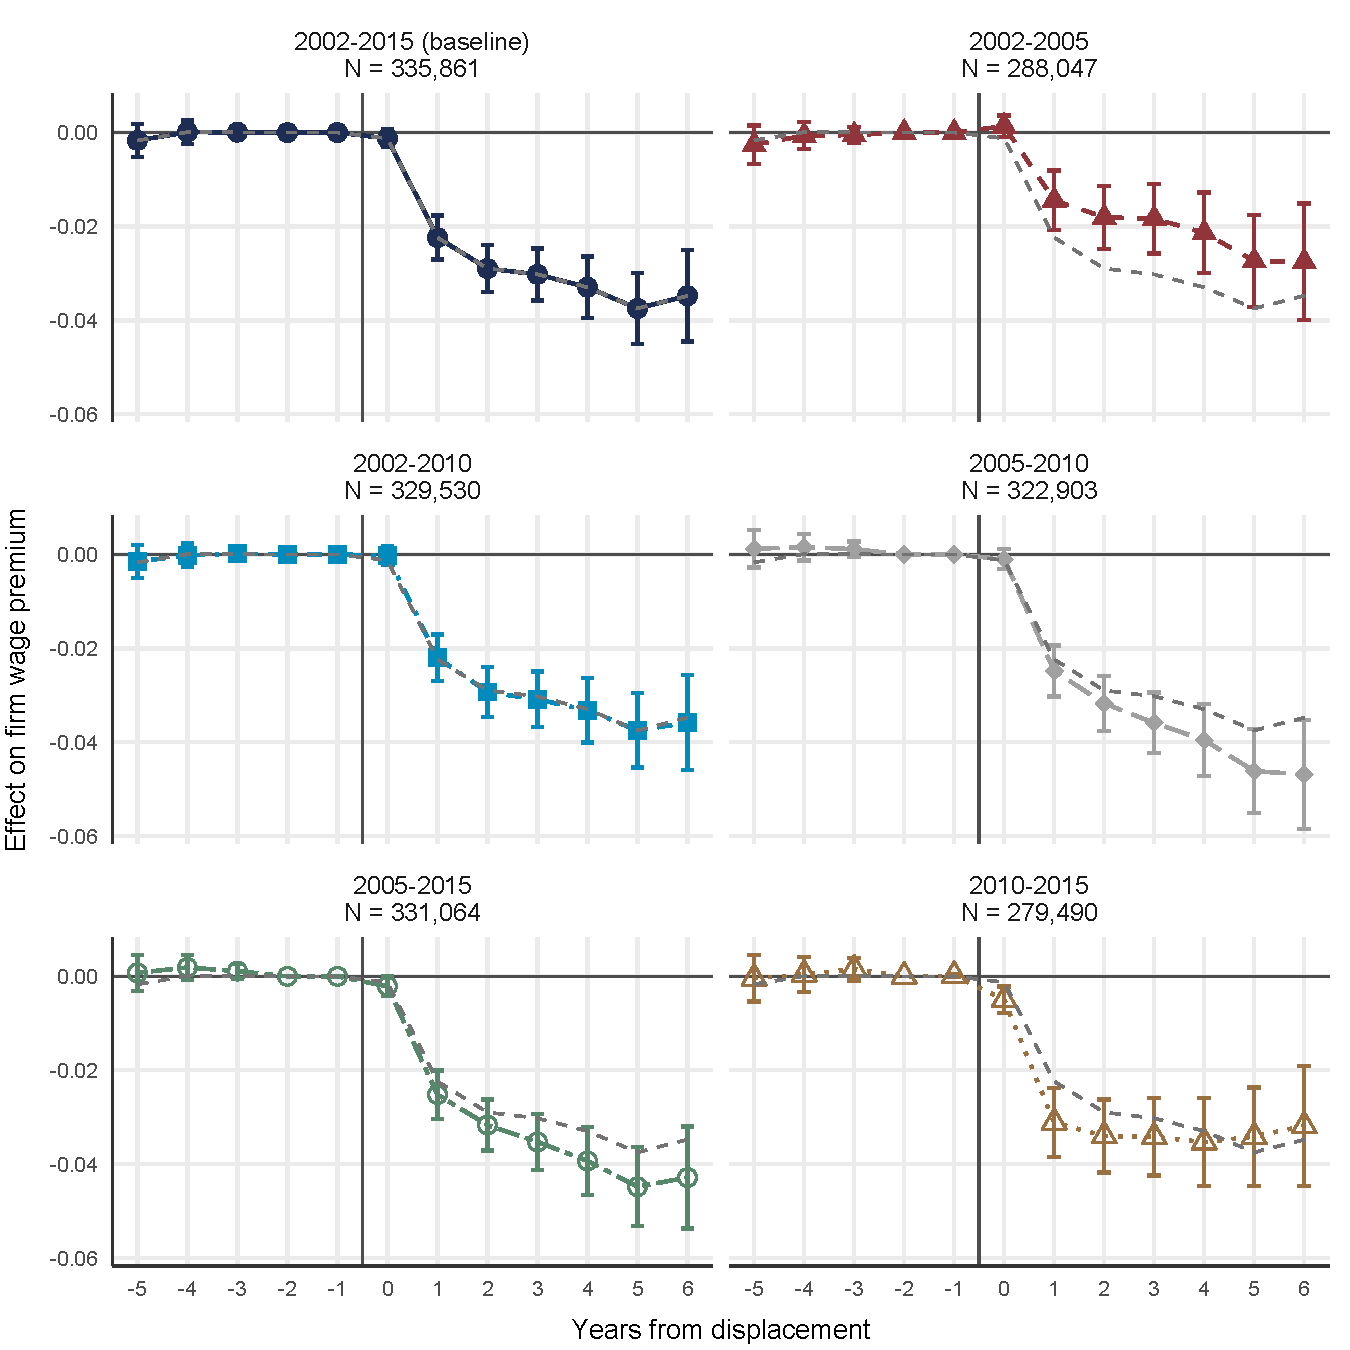
\includegraphics[width=0.95\linewidth,height=0.7\textheight,keepaspectratio]{../figures/03_akm_periods/figure_A5_akm_estimation_windows.pdf}

\par\medskip
\begin{minipage}{0.95\linewidth}\footnotesize\justifying\textsc{Notes}: Event-study estimates of the effect of job displacement on the firm wage premium of the current employer (equation~\ref{eq:main_estimating_equation}), for the LE sample. In each panel, the AKM firm fixed effects are estimated over the window indicated in the title; the top-left panel (2002--2015) is the baseline of Figure~\ref{fig:fe_current_event} of the paper, and is reproduced as a dashed grey line in the other panels. $N$ is the number of worker-year observations; it varies across windows because the set of firms with an estimated premium changes with the window. $t^D-2$ is the reference period. Standard errors are clustered at the worker level.\end{minipage}
\end{figure}


\end{document}
